The Team Zero Chat Application consists of various parts, as determined in the Design section previous. These are the Server, PostgreSql database, Web client, and Android client, the implementation details of which are all described in their respective sections below. Each team member was in charge of one part of the system to implement, although we still worked on parts together as a team as well.

The Team Zero Chat Application itself can be found on the GitHub repository at \\
\url{https://github.com/MetallicFocus/team_zero_application.git}.

Before delving into each individual section of the Team Zero Chat Application, it is important to note how the overall implementation has deviated from the requirements specification in section \ref{requirements}. 

\subsubsection{Deviations from requirements in implementation}
\label{deviations-from-requirements}

Any deviations to priorities or order of implementation were due to various reasons such as previously unforeseen dependencies, and implementation or integration difficulties. Some requirements were not implemented due to time constraints.
The requirements that were not implemented due to time constraints are the following:
\begin{itemize}
\item 2.2. To send an email on registration to validate email address - At present, there is only front-end validation of email address format.
\item 4.1. User and group avatars/pictures
\item 4.2. Multimedia messages (note: emoticon messages do send but this currently depends on whether the client device encoding allows for it)
\item 4.4. QR code for adding new friends 
\end{itemize}

The requirements that were partially implemented are the following:
\begin{itemize}
\item 2.1. Group chat functionality
\end{itemize}

Group chat functionality was implemented in the server and the web client. 

The server supports and provides an API for clients to create, search, join (or leave), and send messages in group chats. However, due to time constraints, and because we chose to prioritise implementation of a secure system with good encryption protocols, Android client does not yet implement the group chat functionalities. However, this is something that could be extended given some time as the API already exists.

\section{Server}
\subsection{Implementation}

The server was implemented as a text based Java application, running the latest (at the time of writing) version of Java (v13) using the Eclipse integrated development environment.

The Server can connect to a client via a web socket, given the correct IP address and the port number 1234 (at the time of writing). When a client tries to connect to the server, the web socket protocols will send confirmation of the successful or unsuccessful connection between the two to both parties. Currently, this connection between the client and server is not a secure one. 

Once connected, the Team Zero Server has it's own interface to interpret client communication requests, which must entirely be in JSON format. These utilize the web socket frameworks 'sendMessage' and 'onMessage' calls to send the data across. Sections \ref{requestsToServer} and \ref{repliesFromServer} below describe all possible requests to and replies from the server.

The server uses three external libraries: \verb|java-json|, to read and write JSON objects; \verb|java-websocket-1.3.0|, to use web socket server functionality; and \verb|posgresql-42.2.8| to use functions to connect to the PostgreSQL database.

The implementation consists of various classes, each with their own set of functionalities summarised below.

\textbf{ServerMain}, the main entry point of the system, is in charge of client communication (it extends the Web Sockets framework as a web socket server), parsing JSON requests, generating JSON replies, as well as keeping track of  a message texts that need to be sent to currently offline clients (using HashMaps). It keeps track of client communications by keeping a HashMap of Websocket to Client IDs, and communicates with a ClientManager to keep track of which clients are currently online. It also sets up a Logger that outputs to the console as well as to a ServerLog.txt file for troubleshooting and debugging purposes. 

\textbf{DbConnection} has all the methods that will require a connection to the postgresql database such as adding users or messages, checking a user's authentication status, retrieving chat histories, or searching for usernames given a query. It connects directly to the database which is deployed on Heroku using a hardcoded address, username, and password. Only one DbConnection object is used per websocket connection, which is always called from ServerMain, to avoid inconsistencies or issues with database connections.

One particularly challenging task was to write the method to search for groups given a query, as this required a more complex PostgreSQL query than the other methods due to the way that the users and groups were linked by their referenced IDs (see figure \ref{db-schema}). In addition to getting the group names that fit the query, we also wanted to get a list of all the members in the group, which took several weeks to figure out. See figure \ref{search-group} solution below.

\begin{figure}[H]
  \frame{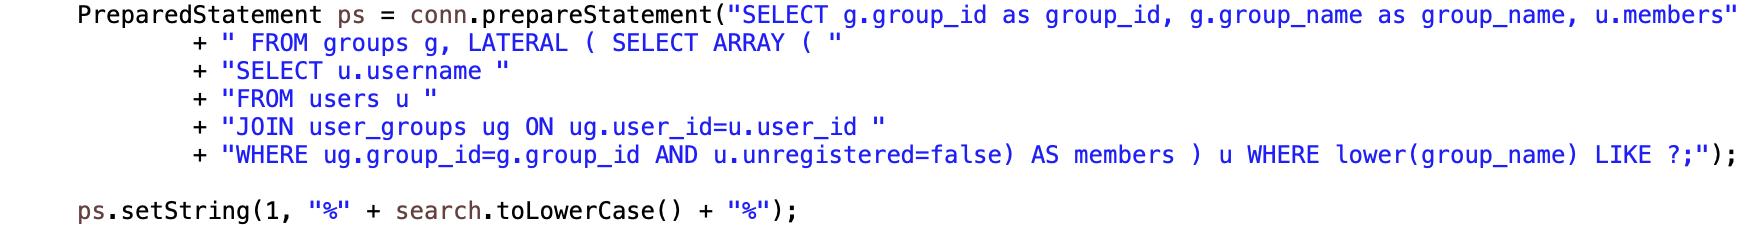
\includegraphics[width=\linewidth]{images/getSearchedGroupsCropped.png}}
  \caption{The getSearchedGroups method in DbConnection.java, the solution to a particularly difficult problem}
  \label{search-group}
\end{figure}


\textbf{Client} simply encapsulates a client user, and has fields such as username, id, email, publicKey, and a flag that states whether or not they are logged in.

\textbf{Group} simply encapsulates a group, and has fields such as group id, groupName, an array of group members and an array of members that left the group.

\textbf{ClientManager} is a singleton class that contains a HashMap to keep track of clients and specify which are online. As it follows the singleton design pattern, only one instance of this class can exist, so any time it is called on we can be sure that it is kept consistent and there will be no concurrency issues. The ClientManager is used by both ServerMain and DbConnection to determine when a client is online. ServerMain adds a client to the ClientManager when they Login, and removes them when the client closes the connection. DbConnection uses it to check whether a client is online or not when returning lists of clients. 

\textbf{ChatMessage} encapsulates a chat message, and has fields such as time sent, and username of the sender and recipient. 


\subsection{Database}

The Team Zero Server Database was implemented using PostgreSql and consists of 6 tables, as seen in figure \ref{db-schema} below.

\begin{figure}[H]
  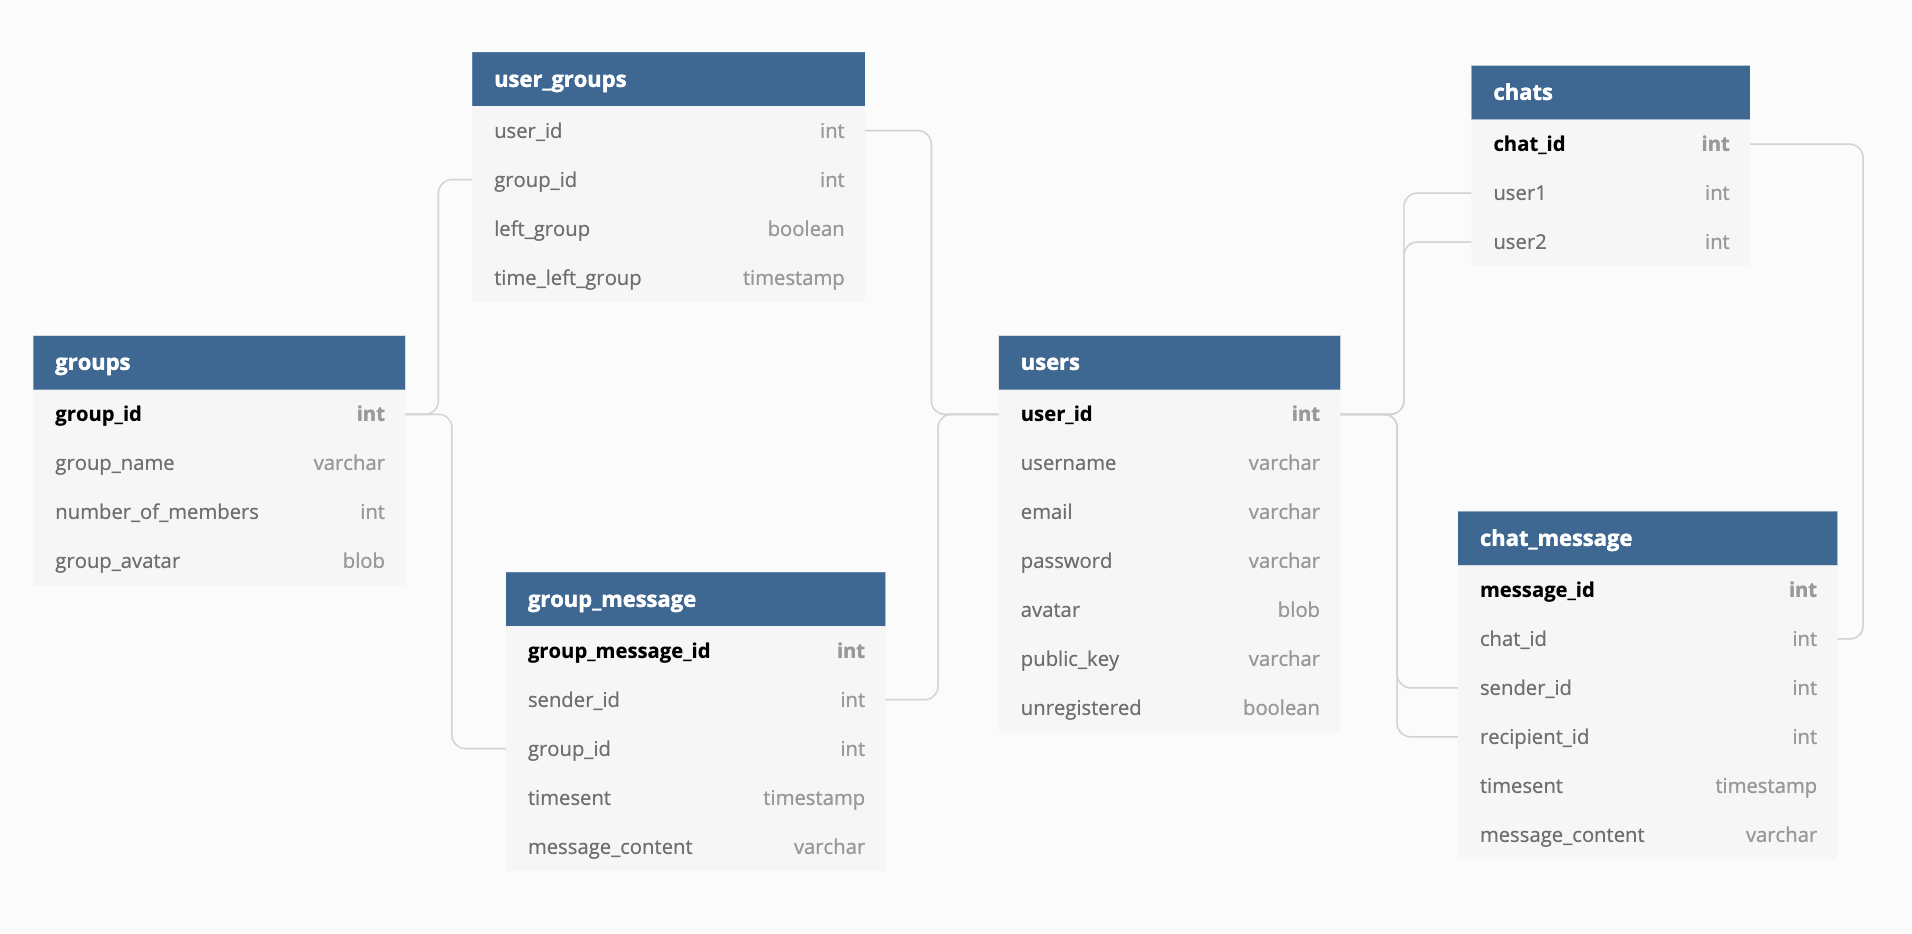
\includegraphics[width=\linewidth]{images/db.png}
  \caption{The Team Zero Server Database schema}
  \label{db-schema}
\end{figure}

A ``user" in the Team Zero Database is the same as a ``client" in Team Zero Server. This difference in terminology was agreed on due to the slight nuances in meaning - the database is referring to the individuals using the system, and the server is referring to the devices connected at the moment in time (even though they are one and the same at that moment in time).

Although the schema for the database was determined prior to implementation, there was generally not much need for change once implementation started. There was one main issue that required change, which was that once a user had sent any chat messages, their \verb|user_id| would become a required foreign key constraint, and the user would no longer be able to be deleted if they wished to unregister. This caused a problem once messaging functionality was implemented, as unregister tests began failing due to the database being unable to delete the user entry. We solved this issue by deciding to add an \verb|unregistered| flag to the \verb|users| table, setting it to true only if a user requests to unregister, and only including users with \verb|unregistered=false| entries in other queries. This same situation applied to group members leaving a group chat as well.


\subsection{Deployment to Heroku}

The database was deployed to Heroku, a cloud platform, to allow all group members to access and use it for testing purposes at any time. The data within the database can be viewed using the Pg Admin 4 software, which was also essential to our testing efforts.

We initially planned to also deploy the Team Zero Server application to Heroku as well, but unfortunately came across difficulties and decided to prioritise time on implementation, as local servers could be run on any machine for testing. 


\subsection{Server Interface for Client Communication (The API)}

\subsubsection{Requests accepted by Server}
\label{requestsToServer}


\begin{table}[H]
        \centering
        \small
        \setlength\tabcolsep{5pt}
\scriptsize
\begin{tabular}{ |c|c|c| } 
 \hline
 \textbf{Request type} & \textbf{Parameter} & \textbf{Parameter} \\
 \textbf{name} & \textbf{Name} & \textbf{description} \\
 \hline
 REGISTER & \verb|username| & User's username to register  \\ 
 & \verb|password| & Password associated with the username
 \\  &\verb|email|& User's email address
 \\  &\verb|picture|& User's profile picture
 \\  &\verb|publicKey|& User's public encryption Key
 \\  
  \hline
  LOGIN & \verb|username| & Username to login with  \\
  &\verb|password|& Password associated with username\\ 
  \hline
 TEXT & \verb|fromUsername| & Username of user sending the text message  \\ 
   & \verb|toUsername| & Username of intended recipient user
  \\  & \verb|message| & The text message \\ 
  \hline
 GETALLCONTACTS &  &   \\ 
  \hline
 SEARCHCONTACTS & \verb|search| & The search query \\ 
  \hline
 EDIT & \verb|username| & Username of editing user  \\ 
 &\verb|newPicture|& New profile picture to update \\
 &\verb|publicKey|& New public encryption key to update \\  
  \hline
 GETCHATHISTORY & \verb|myUsername| & Username of requesting user  \\ 
 &\verb|theirUsername|& Username of contact to get chat history of \\
 &\verb|historyDays|& how many days (int) of chat history to get \\  
  \hline
 UNREGISTER & \verb|username| & Unregistering user's username  \\ 
  &\verb|password|& Password associated with username \\ 
 \hline
 GETPUBLICKEY & \verb|username| & Username of the user whose public key is requested \\ 
  \hline
 CREATEGROUP & \verb|username| & Username of user creating the group  \\ 
   & \verb|groupName| & Name to give to group \\ 
  \hline
 JOINGROUP & \verb|username| & Username of user joining the group  \\ 
   & \verb|groupName| & Name of group to join \\ 
  \hline
 GROUPTEXT & \verb|sender| & Username of user sending the message \\ 
 &\verb|groupName|& Name of group to send the message to \\
 &\verb|messsage|& The text message \\  
  \hline
 GETALLGROUPS &  &   \\ 
  \hline
 SEARCHGROUPS & \verb|search| & The search query  \\ 
 \hline
  GETGROUPHISTORY & \verb|myUsername| & Username of requesting user \\ 
 &\verb|groupName|& Name of group to to get the history of \\
 &\verb|historyDays|& how many days (int) of chat history to get \\  
  \hline
  GETALLUSERGROUPS & \verb|myUsername| & Username of requesting user \\ 
  \hline
  REMOVEGROUPMEMBER & \verb|myUsername| & Username of requesting user \\ 
 &\verb|groupName|& Name of group to exit \\  
  \hline
  SEARCHUSERSNOTINGROUP & \verb|search| & The search query \\ 
 &\verb|groupName|& Name of group to search for users in \\  
  \hline
\end{tabular}
\end{table}



Notes:
\begin{itemize} 
\item UNREGISTER does not delete a user, it only sets a flag in the database. This allows their chat messages to remain in other users' chat histories. However, their username and email cannot be used again for a new registration.
\item GETCHATHISTORY will return the chat history in order with most recent history first.
\item Once a user creates a group, they automatically join the group - there is no need to separately do a JOINGROUP request.
\item GETGROUPHISTORY will return the group chat history in order with most recent history first and if the user requesting the history is not part of the group, it will return the group chat history till the time they were part of the group.
\item REMOVEGROUPMEMBER does not delete a user from a group, it only sets a flag in the database and sets the time of exit. This allows their group chat messages to remain in other users' group chat histories and allows this user to view the chat history of the group they left till the time they were inside the group. However, they can't be added again to the group.
\item The server keeps a HashMap object of any TEXT or GROUPTEXT messages awaiting sending (to clients who are not currently connected) and will send them on connection. In the case of several messages to be sent on connection, each message is sent separately with 10ms of sleep in between to avoid overloading the clients and causing them to crash (this 10ms of sleep was introduced after some integration tests which caused clients to crash).
\end{itemize}

%See Appendix \ref{requestToServerAppendix} for how these requests should be used with the given parameters in a JSON string, for the server to accept them.

\subsubsection{Replies returned from Server}
\label{repliesFromServer}



\begin{table}[H]
        \centering
        \small
        \setlength\tabcolsep{5pt}
\scriptsize
\begin{tabular}{ |c|c|c| } 
 \hline
 \textbf{Reply} & \textbf{Parameter} & \textbf{Parameter} \\
 \textbf{From} & \textbf{Name} & \textbf{description} \\
 \hline
 LOGIN & \verb|reply| & states which reply type it is and whether it was a success\\ 
 REGISTER &  &   or failure  \\ 
 EDIT & \verb|message| & an optional status message  \\ 
 UNREGISTER &  &  \\  
 CREATEGROUP &  &  \\  
 JOINGROUP &  &  \\  
  \hline
  TEXT & \verb|sender| & Username of text message sender  \\
  &\verb|recipient|& Username of text message recipient \\ 
  & \verb|message| & Text message   \\ 
   & \verb|timestamp| & Time received at server in format yyyy-MM-dd HH:mm:ss \\ 
  \hline
 GETALLCONTACTS & \verb|reply| &  states whether it was a success or failure \\ 
  & \verb|contacts| &  A JSON array of User information \\ 
  \hline
 SEARCHCONTACTS & \verb|reply| &  states whether it was a success or failure \\ 
  & \verb|contacts| &  A JSON array of User information \\ 
  \hline
 GETCHATHISTORY & \verb|reply| &  states whether it was a success or failure \\ 
  & \verb|messages| &  A JSON array of message information \\ 
  \hline
 GETPUBLICKEY & \verb|reply| &  states whether it was a success or failure \\ 
  & \verb|username| &  username of the associated public key \\ 
  & \verb|publicKey| &  Public encryption key in base 64 format \\ 
  \hline
 GETALLGROUPS & \verb|reply| &  states whether it was a success or failure \\ 
  & \verb|contacts| &  A JSON array of Group information (name and members) \\ 
  \hline
 SEARCHGROUPS & \verb|reply| &  states whether it was a success or failure \\ 
  & \verb|contacts| &  A JSON array of Group information (name and members) \\ 
  \hline
  GETALLUSERGROUPS & \verb|reply| &  states whether it was a success or failure \\ 
  & \verb|contacts| &  A JSON array of Group information (name and members) \\ 
  \hline
  GROUPTEXT & \verb|sender| & Username of text message sender  \\
  &\verb|groupName|& Name of group message was sent to \\ 
  & \verb|message| & Text message   \\ 
   & \verb|timestamp| & Time received at server in format yyyy-MM-dd HH:mm:ss \\ 
  \hline
  GETGROUPHISTORY & \verb|reply| &  states whether it was a success or failure \\ 
  & \verb|messages| &  A JSON array of message information \\ 
  \hline
  REMOVEGROUPMEMBER & \verb|reply| &  states whether it was a success or failure \\ 
  & \verb|messages| &  An optional status message \\ 
  \hline
  SEARCHUSERSNOTINGROUP & \verb|reply| &  states whether it was a success or failure \\ 
  & \verb|messages| &  A JSON array of User information \\ 
  \hline
 
\end{tabular}
\end{table}


%See Appendix \ref{dataReturnedFromServerAppendix} for how these requests should be used with the given parameters in a JSON string, for the server to accept them.



\subsubsection{Possible error replies from Server}
\label{api}

\begin{table}[H]
        \centering
        \small
        \setlength\tabcolsep{5pt}
\scriptsize
\begin{tabular}{ |c |c|c| } 
 \hline
 \textbf{Possible error reply from} & \textbf{Situation} & \textbf{Possible response message } \\
 \hline
 REGISTER & User uses an existing username & ``Username already exists"  \\ 
 & User uses an existing email & ``Email already exists"
 \\  
  \hline
  LOGIN & incorrect username or password & ``Cannot authenticate user. \\
  &&Check login details."  \\
   \hline
 TEXT & User did not log in & ``Sender is not logged in"   \\ 
  \hline
 GETALLCONTACTS & User did not log in & ``User is not logged in" \\ 
  \hline
 SEARCHCONTACTS & User did not log in  & ``User is not logged in" \\ 
  \hline
 EDIT & User did not log in & ``User is not logged in" \\
  \hline
 GETCHATHISTORY  & User did not log in & ``User is not logged in"  \\
  \hline
 UNREGISTER  & User did not log in & ``User is not logged in"  \\ 
 \hline
 GETPUBLICKEY & Bad username given & ``No user found with given username"  \\ 
 \hline
 CREATEGROUP & User did not log in & ``User is not logged in" \\
 & User gives an existing group name & ``Groupname already exists"  \\ 
 \hline
 JOINGROUP& User did not log in & ``User is not logged in" \\
  & User gives a nonexistant group name & ``Group name does not exist"  \\ 
 \hline
 GETALLGROUPS& User did not log in & ``User is not logged in" \\
 \hline
 SEARCHGROUPS & User did not log in & ``User is not logged in" \\ 
 \hline
 GROUPTEXT & User did not log in & ``User is not logged in" \\
 & Either a username or group name is bad & ``No such group with member in it"  \\ 
 \hline
 GETGROUPHISTORY  & User did not log in & ``User is not logged in"  \\
  \hline
  GETALLUSERGROUPS& User did not log in & ``User is not logged in" \\
 \hline
 REMOVEGROUPMEMBER  & User did not log in & ``User is not logged in"  \\
  \hline
  SEARCHUSERSNOTINGROUP& User did not log in & ``User is not logged in" \\
 \hline
 Other &  Unsupported request name given & ``unrecognised type"  \\ 
 & Unparsable string (Not JSON compliant) & ``bad JSON Format"\\ \hline
 Database issue & internal bug & SQLException message\\ 
  \hline
\end{tabular}
\end{table}


\subsection{Testing with a Test Client}

As the server implementation involves many interconnected parts and requires a websocket connection to access ServerMain, the ServerTesterClient was implemented to test individual functionalities to be as close to unit testing as possible. The client is a text based Java application which connects to the server using the websocket protocols, and sends JSON requests to perform tests as required. The output of this client can be analysed and checked against the server's logs to see if the messages received are as expected. 

Each request and reply outlined in section \ref{api} above was tested in various scenarios using the test client, including tests that expected error replies based on situations such as trying to create a new group and giving an existing group name. Testing was done throughout implementation, during and after each feature implemented, and included checking for potential bugs in previously implemented features as well. 

Figure \ref{clientTest} below shows a sample output from the ServerTesterClient.


\begin{figure}[H]
  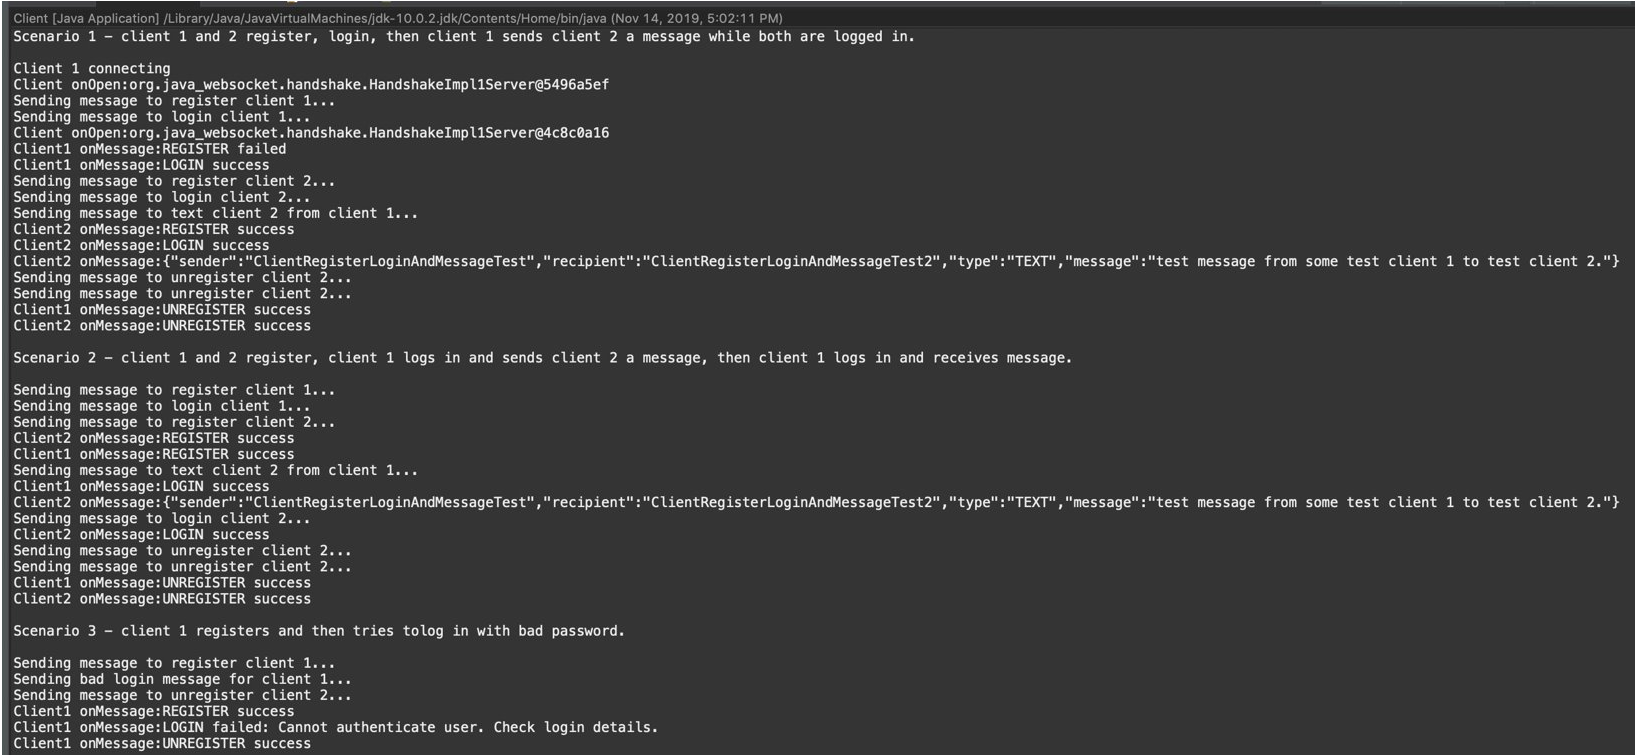
\includegraphics[width=\linewidth]{images/clientTest.png}
  \caption{Sample output from the ServerTesterClient}
  \label{clientTest}
\end{figure}

\label{server}

\section{Web client}

\subsection{Technologies}

Web clients were implemented on Node.js, with Vue and Element as javascript component libraries, and Crypto and CryptoJS as encryption tools.

\begin{itemize}
    \item \textbf{Runtime:} Node.js 6.13.4
    \item \textbf{Dependencies:} Vue 2.6.10; Element 2.13.0; Crypto 1.0.1; CryptoJS 2.1.3
\end{itemize}

Node.js is an asynchronous event-driven JavaScript runtime. With non-blocking calls, it is designed to build scalable network applications, which implements concurrency model\cite{nodejs}\cite{non-blocking}. Because of such a feature, a large number of open-source modules were built upon Node.js. To make use of these modules, Node.js was chosen to be used in this project.

Vue is a progressive framework for building user interfaces. The core library is focused on the view layer only, and is easy to pick up and integrate with other libraries or existing projects \cite{vue}. Element is a Vue 2.0 based component library. Most basic functions were implemented using Vue, especially when considering responsive data and components. To effectively construct a neat html page, components like chatting panel were pre-constructed to be rendered and inserted when needed. As an auxiliary tool for Vue, Element provided a variety of content-independent components together with fancy styles.

Crypto is an embeded crypto library of Node.js. We meant to utilize Crypto to implement all functionalities about encryption and decryption. However, AES related functions of Crypto did not work well with this project (it was missing some functions), so we turned to another library called CryptoJS. As a result, Crypto was used to generate Diffie-Hellman public and private keys during registration and to calculate shared secrets on initialising new chats, completing the functionality of key exchange. CryptoJS was used to do message encryption and decryption using AES with the previously computed shared secret key.


\subsection{Implementation}

Inspired by MVVM model, Vue provides an API for data binding. It is also called declarative rendering in \cite{vue}, because Vue pages preserve a section for data object storage that is realized by variable declaration, and binding is between these data objects and DOM objects. Besides, Vue data objects are written in a similar form as JSON, which means it easier using Vue to communicate with the Server. 

Web clients connect to the server through WebSocket in Web API, listening to predefined port, and communicating in the form of JSON requests and responses. If websockets are supported by a user's browser, the process of websocket initialisation done by \texttt{initWebSocket()} will be triggered once the pages are rendered. This is completed in \texttt{mounted()}, a predefined function of .vue files. In addition, the websocket connection will automatically close immediately after page destruction.

With constructed JSON requests, web clients use \texttt{this.websocket.send(this.request)} to forward it to the server. Since there is a latency to receive responses, web clients would get nothing when trying to parse JSON responses immediately after sending requests. Thus, a section named \texttt{watch} defined by Vue was exploited. It was to monitor any change on data objects and do reactions towards changes. only if responses are sensed and received from websocket will clients start to parse responses and do further actions.

Responses are stored in the data object called \texttt{response} with a sentence \texttt{this.response = event.data}. Once the change was detected, \texttt{watch} would parse the response with sentence \texttt{this.parsed\_response = JSON.parse(newR)} from JSON into Vue data objects. Afterwards, web clients can use the operator "\texttt{.}" to directly fetch related attributes that are consistent to the server. Figure \ref{tab:code-example} shows an example of how web clients deal with responses about messages from the server. It abstracts arguments from \texttt{parsed\_response} and pass them to \texttt{getNewText(sender, message)} to perform actual operations.

\begin{figure}[H]
 \centering
  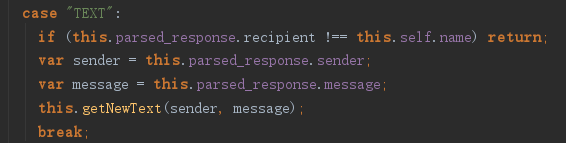
\includegraphics[width=0.8\textwidth]{images/code-example.png}
  \caption{Example of Operations on Responses}
  \label{tab:code-example}
\end{figure}

When using Vue components, we do not need to create DOM objects directly, such as \texttt{let newDiv = document.createElement("div")} but pass this job downwards. That is to say, if a new message was caught and corresponding UI was to be generated, the only thing we had to do was passing data to the pre-constructed component of message box. And it was the component itself that would decide how to present the data.

There are only two pages, \texttt{Signin.vue} and \texttt{Signup.vue}. The format of these files complied to Vue API.

As suggested by the name of \texttt{Signup.vue}, it was designed to handle registration of users. An agreement of registration constrains across both web and android was previously set, and details were described in \ref{android-implementation}. Web clients always check legality of input before constructing JSON requests of registration.

For \texttt{Signin.vue}, both login function and other main functions were integrated in one page. And users can only reach profile and chat information after successful login. Since functionalities of chat rely more on UI, reusable components were introduced in \texttt{Signin.vue}, so that redundant html codes could be omitted and replaced by particular function (i.e. for loop function).

\subsubsection{Components}

A table as follows shows the reusable components constructed in web clients.

\begin{table}[H]
\scriptsize
\begin{center}
\begin{tabular}{|c|c|}
\hline
\textbf{Components}             & \textbf{Description}                                                                                                                                                                                           \\ \hline
\texttt{single-chat.vue}                & \begin{tabular}[c]{@{}c@{}}A chat card in the contact list\\  indexing corresponding chat panel.\end{tabular}                                                                                                  \\ \hline
\texttt{group-chat.vue}                 & \begin{tabular}[c]{@{}c@{}}A group chat card in the contact list \\ indexing corresponding group chat panel.\end{tabular}                                                                                      \\ \hline
\texttt{single-chat-panel.vue}          & \begin{tabular}[c]{@{}c@{}}A chat panel showing decrypted messages\\  between two particular users. It may contain\\ \texttt{single-message-from-self.vue} and\\ \texttt{single-message-from-object.vue}.\end{tabular}           \\ \hline
\texttt{group-chat-panel.vue}           & \begin{tabular}[c]{@{}c@{}}A chat panel showing decrypted messages \\ among members of one particular group. \\ It may contain \texttt{single-message-from-self.vue} \\ and \texttt{single-message-from-group.vue}.\end{tabular} \\ \hline
\texttt{single-message-from-self.vue}   & \begin{tabular}[c]{@{}c@{}}A box showing one decrypted message together\\  with sending time from the authorised user.\end{tabular}                                                                            \\ \hline
\texttt{single-message-from-object.vue} & \begin{tabular}[c]{@{}c@{}}A box showing one decrypted message together \\ with sending time from the other in one chat.\end{tabular}                                                                          \\ \hline
\texttt{single-message-from-group.vue}  & \begin{tabular}[c]{@{}c@{}}A box showing one decrypted message from another\\  in one group chat, with time and related user name.\end{tabular}                                                                \\ \hline
\texttt{single-user-info.vue}           & \begin{tabular}[c]{@{}c@{}}A card shown in search user panel, specifying\\  user name, user email address and online status.\end{tabular}                                                                      \\ \hline
\texttt{single-group-info.vue}          & \begin{tabular}[c]{@{}c@{}}A card shown in search user panel, \\ specifying group name.\end{tabular}                                                                                           \\ \hline

\end{tabular}
\caption{Component Description}
\label{tab:component-table}

\end{center}
\end{table}

As shown in the above table, components can be nested (e.g. \texttt{single-chat-panel.vue} may contain \texttt{single-message-from-self.vue} and \texttt{single-message-from-object.vue}), which enhances their usability and convenience.The relation between components and UI and relation among components were depicted more clearly and intuitively in Figure \ref{tab:main-panel-of-user-chat} and Figure \ref{tab:main-panel-of-group-chat}.

\begin{figure}[H]
 \centering
  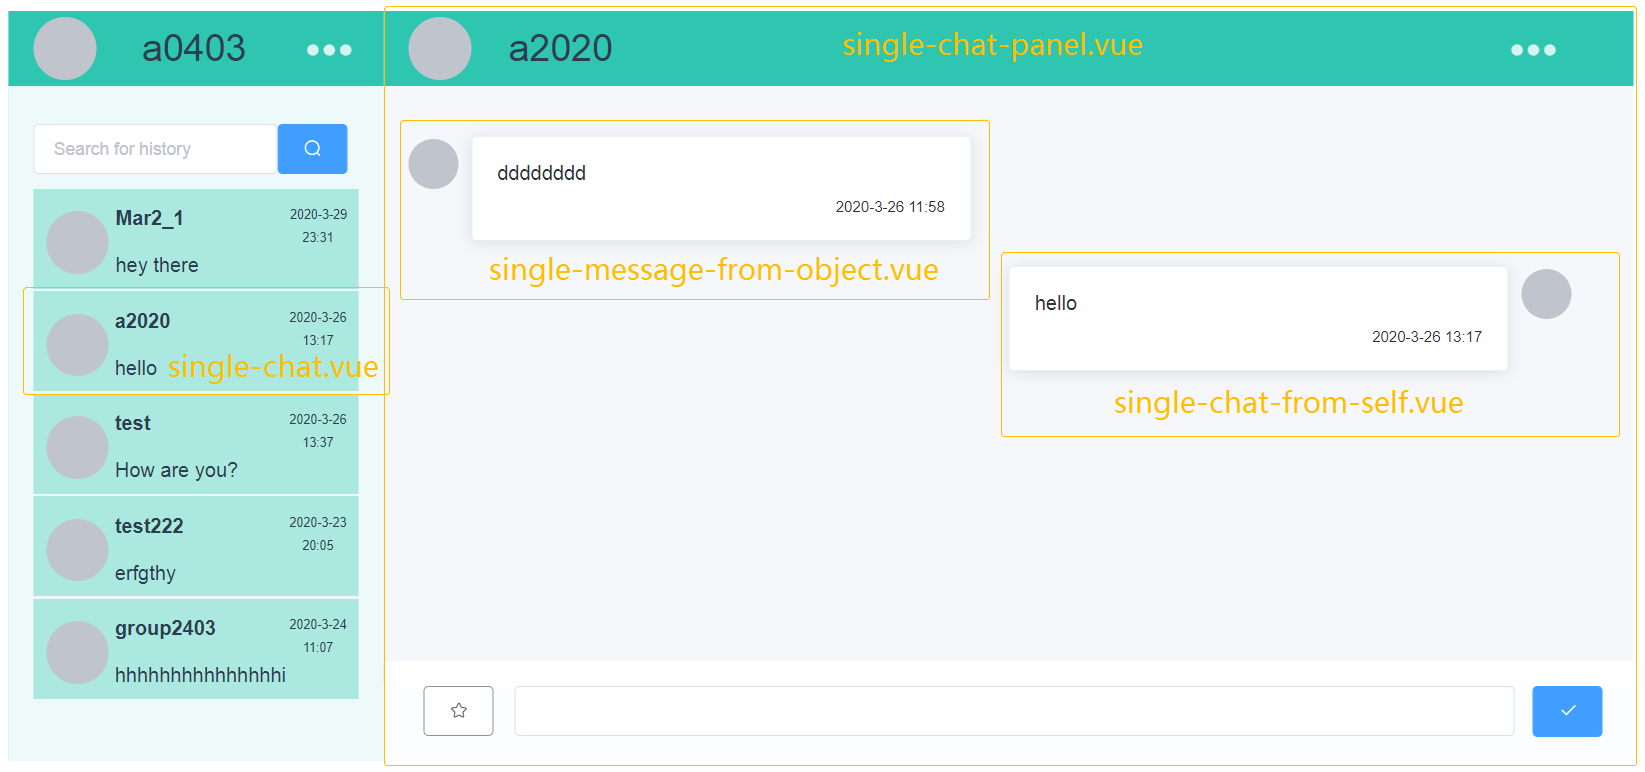
\includegraphics[width=1\textwidth]{images/user.png}
  \caption{Main Panel of User Chat}
  \label{tab:main-panel-of-user-chat}
\end{figure}

\begin{figure}[H]
 \centering
  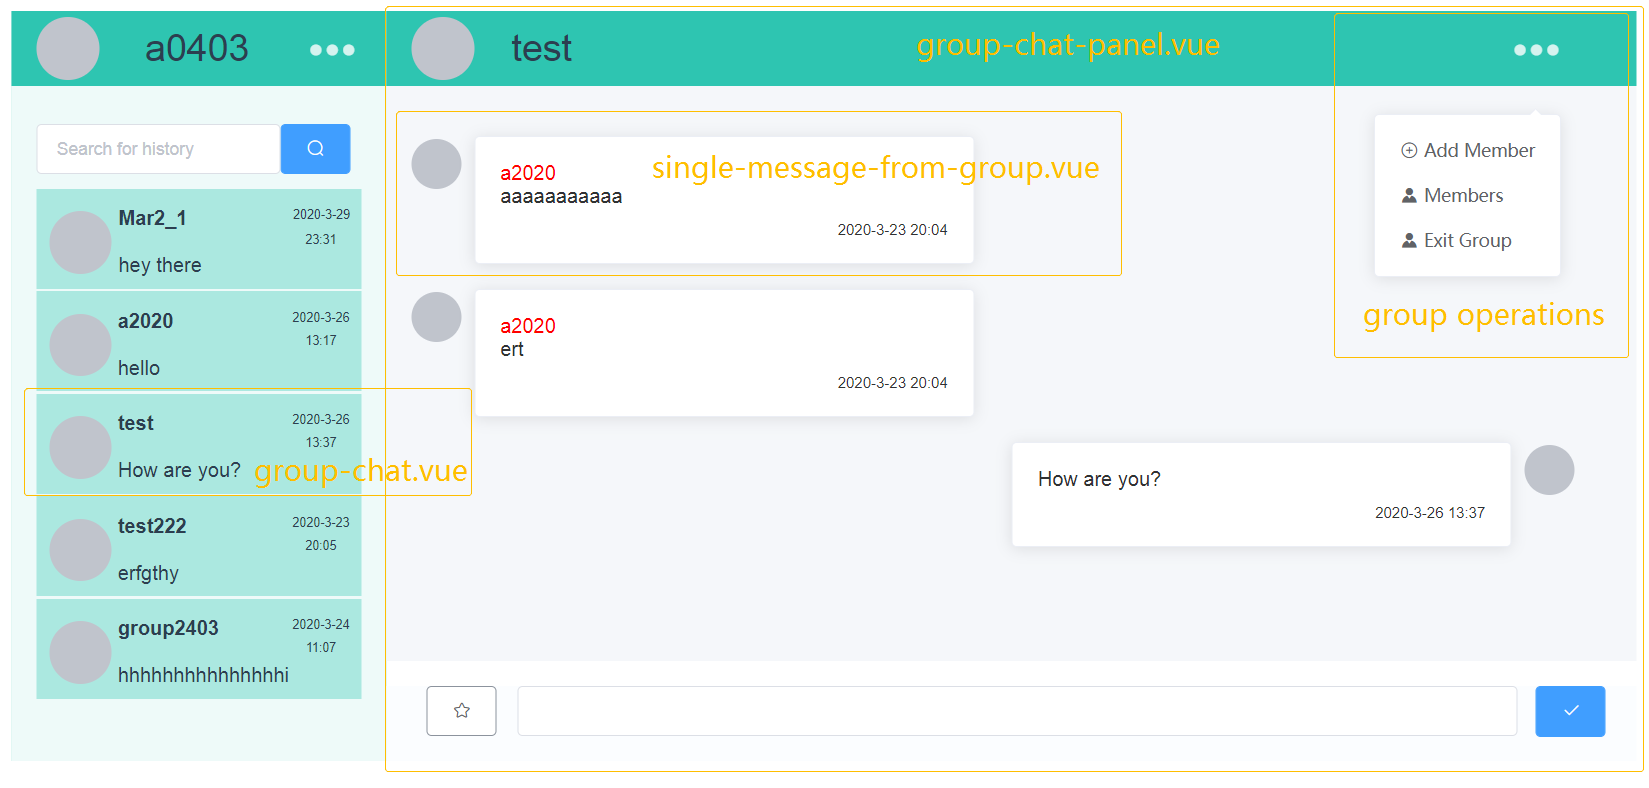
\includegraphics[width=1\textwidth]{images/group.png}
  \caption{Main Panel of Group Chat}
  \label{tab:main-panel-of-group-chat}
\end{figure}

There are more operations hidden in the "..." beside the user name, such as search users, search groups and create groups. Below it is a contact list, the list of users and groups that the concerned user can talk to. 

Each chat card in the contact list corresponds to one particular chatting panel and only one panel would be shown at a time. Since panels will be constructed and rendered previously once a new chat is created, it is fast to display them when needed without further loading. Upon one chat card, the last message content is presented as well as its sending time. Chatting panels present messages from last 24 hours and sorted temporally. For group chat messages, an extra information of sender user name is attached to each message box from others.

More group operations are in the "..." of group chatting panel. As shown in Figure \ref{tab:main-panel-of-group-chat}, they include adding group members, viewing current members and quitting the group.

There is no limit for requesting a chat, so an authenticated user can chat to anyone without their permissions. Every time when users log in, they need to search for other users and create a chat with them. Web clients will request for one-day chat history automatically but store no chat information on local storage. During this process, encryption techniques of DH key exchange and AES256 are used, which will be explained more in \ref{encryption}.

Upon both login and registration, passwords are hashed locally by MD5 to ensure confidentiality on networks.

\begin{figure}[H]
 \centering
  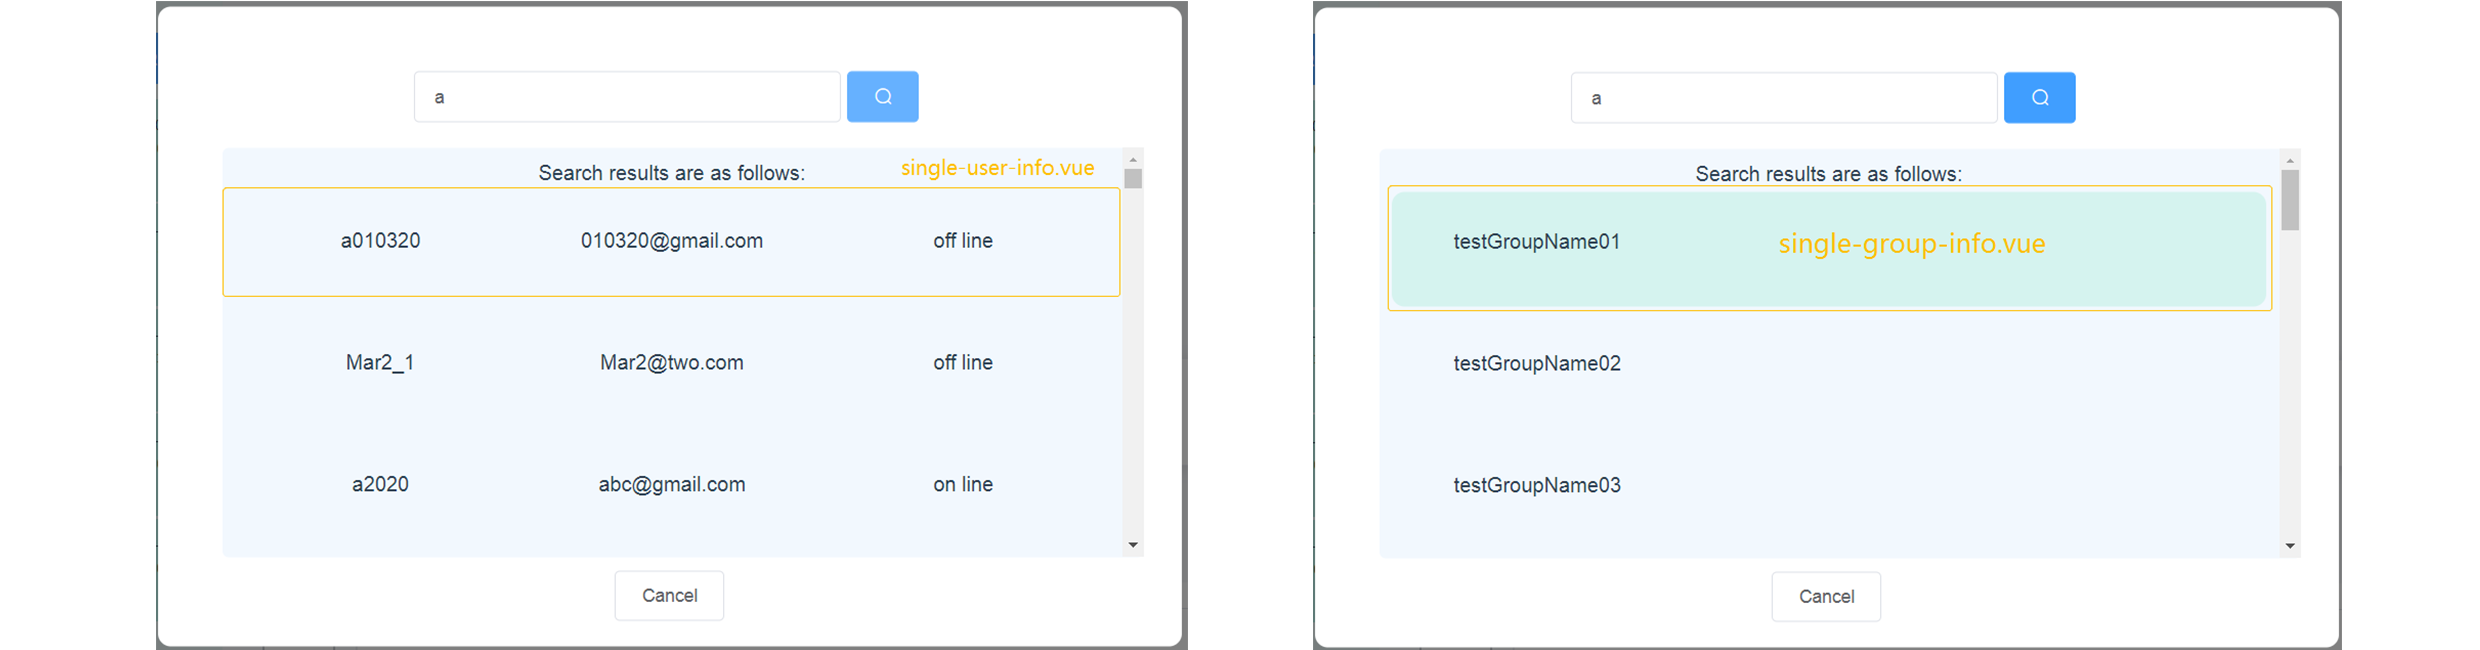
\includegraphics[width=1\textwidth]{images/search.png}
  \caption{Search Panels}
\end{figure}

Search user panel and search group panel can be triggered from the hidden more operations. For search user panel, the user is able to obtain basic information of concerned users. And the user can only create a new chat and start messaging from search user panel by clicking an interested information bar. On the other side, search group panel made use of a different policy. Search group panel only displays the list of searched group names, while the list of groups that the user is in are requested at the beginning after successful login. It is reasonable because the user may not be authorised to join every group. 

\subsection{Automation Testing}

The objective of testing here is to test functionality and usability of website. Automation testing is a testing technique, achieved by writing test scripts or using any automation testing tool to automate repetitive tasks and other testing tasks which are difficult to perform manually\cite{automation-testing}.

Like other testing, automation testing can be classified with respect to the phrase of testing: unit test, API test and UI based test. Among these tests, \verb|unit tests| are commonly run during the development phase. \verb|API tests| are run during the integration phase, before or after the UI layer is built for the application. \verb|UI based tests| are run to test the functionality and business logic of the application from the front end of the application\cite{automation-testing}.

Unit test and API test were implemented manually during the process of development and debugging. Only UI based test was run by automation scripts written with Selenium and Python. Testing file selenium-test.py is put under project directory \texttt{/frontend/src/test/}.

\subsubsection{Testing Environment}

Generally speaking, testing is supposed to be performed on various platforms in order to ensure completeness. However for the reason of limited devices and time, the testing was only finished under the following configuration.

\begin{itemize}
    \item \textbf{Operating system:} Windows 8.1
    \item \textbf{Browser:} Google Chrome 80.0.3987.149
    \item \textbf{Testing tools:} Selenium 6.13.4; JavaScript V8 8.0.426.27; Python 3.5.4
\end{itemize}

During the last year, Windows continued occupying the market of operating system of desktops and tablets\cite{desktop-tablet-os-market-share}. As for browsers, Google Chrome has been owning an overwhelming market share among other browsers from last year and made up 64.45\% in this February\cite{browser-market-share-worldwide}. Therefore, we can assume that such an environment configuration covers situations of the majority of users.

Selenium is an automation tool, providing extensions to emulate user interaction with browsers, a distribution server for scaling browser allocation, and the infrastructure for implementations of the W3C WebDriver specification\cite{selenium-project}. According to the survey sponsored by ToolsQA and conducted by Katalon and KMS Technology, Selenium is the most popular automation tool among over 100 tools reported, and a percentage of 84 of the respondents were using it\cite{automation-tools-survey}. In addition, Selenium provides good support for multiple platforms, browsers and programming languages. Thus, it is preferable to choose Selenium to be the automation tool used in this project.

\subsubsection{Test Cases}

With respect to the requirements we had implemented, the testing functions and test cases were planned to be constructed accordingly. Different from use cases, test cases are constructed to validate that software is working fine for each given instruction and yields required results. A simple list of test cases are classified as follows.

\begin{itemize}
    \item \textbf{Register:} to test validation rules, generation and storage of Diffie-Hellman key pairs and functionality of registration.
    \item \textbf{Login:} to test functionality of login and fetched public keys of other users.
    \item \textbf{User chat operations:} to test functionality of searching users, creating a new chat and message encryption with computed shared secret.
    \item \textbf{Group chat operations:} to test functionality of searching groups, creating groups and leaving groups.
\end{itemize}

\subsubsection{Test Results}

Due to time limit, not all of test cases were implemented as planned. Web clients perform good on reacting to registration of both legal and illegal request. Login inputs were not checked before requesting as registration does, but the functionality of login was implemented as required. Only users with private keys stored in local storage can login successfully. As for user chat operations, creating a new chat from search panel proved to work well after testing with no error by repeating searching users, entering search keywords and clicking a random user to start a chat. Since web clients could send encrypted messages and decrypt messages properly from other users, message encryption and decryption were believed to be implemented as console log did suggest messages in JSON requests were not plain text.

Automation testing of group chat operations were not performed yet, but successful cases were used manually to test related functionalities with positive result.

\subsection{Challenges and Drawbacks}

\begin{itemize}
    \item \textbf{Automation testing} Not all test cases were implemented; the automation test of web clients were only able to be performed locally. Though it was originally designed to cooperate with Travis CI, it failed due to the need to use local storage on clients to login and proceed further manipulation.
    \item \textbf{New message notification} There are still some bugs in terms of message notification. To be specific, notification would not appear when a user received a new message from another user not in the current chat list.
    \item \textbf{DH key generation} Although web clients can compute the same shared secret with DH keys generated by CryptoJS, there is a compatibility issue when cooperating with Android clients. The detail is that Web clients generate public and private keys with the same lengths, while Android clients using the \verb|java.security| library generate them with different lengths for some unclear reason.
    \item \textbf{Message encryption on group chat} Group message encryption remains to be implemented because of the difficulty of shared key computation among several users.
\end{itemize}
\label{web}



\section{Android client}
\subsection{Background}

Once every couple of years, there are major changes and breakthroughs in the technological industry. As the ease of information exchange is a key element in our world, the adoption of portable intelligent devices becomes more and more obvious.

Android is one of the major operating systems used in the mobile industry at the moment. International Data Corporation conducted several studies regarding the market share of this operating system during a couple of years. The results depict an astonishing 86.6\% OS share in the world, with a slight increase in the forecast for the next years \cite{android-market-share}. The decision to implement the second client as a mobile application is based on the worldwide popularity of Android. We believe that selecting the leading mobile operating system would bring in a higher amount of possible users.

\subsection{Technologies}
\label{android_technologies}

The main programming language used during the development of the Android application is Java. All of the back-end functionalities along with any front-end code that is dynamically generated in the back-end are done using Java SE 8.

The static front-end is created by using Android native XML code and it is interpreted by the compiler and IDE accordingly.

The mobile application features a local database that is set up using Android Room version 1.1.1. It is a SQLite object library that provides an abstraction level over the database. We have chosen to use Room in order to avoid boilerplate code and efficiently convert SQLite table data into Java objects that can be further manipulated. The reason for the local database is to allow users to view consistent copies of data without the need of a continuous internet connection.

Testing of the application has been completed through an extensive use of both manual and automated testing. For the latter, we have used JUnit 4 framework to write both unit and instrumented tests. More details about how automated tests were designed, implemented and evaluated in the chapter \ref{android_unit_instrumented_testing}

All of the development for this platform has been completed in Android Studio IDE (V 3.5.1). We considered using this IDE instead of others because of its integrated emulating platform on which we could run and test the application in a similar way as installing it onto a real device. The emulator incorporates all the features found on physical devices, from home and volume buttons to settings and its own separate storage. Because it is a considered a different device, the IP address of the emulator is different than the one for the hosting machine. This aspect brings it closer to a real scenario of testing on an actual physical device, as running the server on the same machine as the emulator implies information exchange between different IP addresses.

\subsection{Implementation}
\label{android-implementation}

Implementation of the Android client consists of several back-end Java classes, their respective front-end XML files and a Manifest file (more details below). Besides all of the previous, the Android development provides a different file (\verb|build.gradle|) on which other configurations can be performed. Some of the configurations include the application ID, build type releases, dependencies and target/minimum SDK versions. As part of the build type release, the application uses ProGuard rules that help in shrinking and optimizing the application. At the moment of writing they are turned off, but by changing the \verb|minifyEnabled| property to \verb|true|, ProGuard will shrink the code determined as not required at runtime.

The target SDK version of the app is \verb|level 28| while the minimum SDK version is \verb|level 22|. We have chosen to develop for the \verb|level 28| because it is the level that represents Android 9 (Pie). As of March 2020, approximately 40\% of devices that run on Android use Pie, being the most popular Android version as of now \cite{android-pie-market-share}. 
%The version levels make a difference in the app in the sense that certain libraries as a whole or some specific methods are not available for older versions of the OS. This is why we used {\small\verb|level 22|} as a minimum, to ensure maximum support across a wide range of OS versions while maintaining the same functionalities. 

The Manifest file describes essential information about how the application works. It contains details about package names, app components and permissions. As a standard, the file always has to be named \verb|AndroidManifest.xml|. In terms of permissions, our app needs to connect to the internet for the system communication to take place (\verb|android.permission.INTERNET| allows it to open network sockets).

In terms of app components, we have defined the following activities: \verb|MainActivity|, \verb|Registration|, \verb|ChatList|, \verb|Chat| and \verb|NewChat|. The first one of the batch is the one that will be launched on when the application is opened, so it is marked as \verb|android.intent.action.MAIN|. This tells the operating system that this activity is the main entry point when opening the application. The \verb|ChatList| activity is defined as a \verb|searcheable| activity by using the \verb|SEARCH| action. This is useful for placing queries onto data that is not necessary part of the local database. For instance, the chat lists for each user is retrieved from the DB but using the search property of the activity, queries can be placed on the fetched data, without the need to access the database again.

The activities mentioned above refer to Java classes in the application that directly reference a specific screen. This means that when a user enters a view (in the MVC model), the displayed screen contains back-end functionalities of the specific Java class attached to it. There are more Java classes that act as additional tools, containing methods that are used by the activities. In the following paragraphs, we will write about each class in particular and mention all of the important information for each (regarding what features are contained within them, code details and other interesting facts).

\textbf{MainActivity} is the activity on which the application launches to. It is attached to the \verb|activity_main.xml| front-end layout. It serves as a welcome page containing the \textbf{login prompt} and a button to go to the registration page in case the user wants to register an account. This is also the point in the app when the \textbf{WebSocket connection is initialised} and the persistent connection to the server is established. % Possibly write about user being notified if the server connection is not possible

After credential completion, the login fields are filtered through an internal validation tool that we created. The validation tool is found in the file \verb|RegistrationValidator.java| under the \verb|tools| package. It contains 5 methods that are used both for the login process and the registration process. Its main purpose is to make sure the input from the user is considered valid. This helps in securing the application from SQL injection.

The following table (\ref{tab:login_validations}) contains information about how the login credentials are checked.

\begin{table}[h]
\begin{center}
\scriptsize
\begin{tabular}{|l|l|l|}
\hline
\multicolumn{1}{|c|}{\textbf{Validation}} &
  \multicolumn{1}{c|}{\textbf{Rule}} &
  \multicolumn{1}{c|}{\textbf{Regex Rule}} \\ \hline
\multicolumn{1}{|c|}{\begin{tabular}[c]{@{}c@{}}Username \\ \it{(validateUsername method} \\
\it{in RegistrationValidator.java)} \end{tabular}} &
  The field is not empty &
  \multicolumn{1}{c|}{\begin{tabular}[c]{@{}c@{}}\textbackslash{}\textbackslash{}b{[}a-zA-Z{]}\\ {[}a-zA-Z0-9\textbackslash{}\textbackslash{}-.\_{]}\\ \{3,30\}\textbackslash{}\textbackslash{}b\end{tabular}} \\
 &
  \begin{tabular}[c]{@{}l@{}}No illegal characters \\ (except '-', '.' and '\_')\end{tabular} &
  \multicolumn{1}{r|}{} \\
 &
  Does not start with numbers &
   \\
 &
  Between 3 and 30 characters &
   \\ \hline
\begin{tabular}[c]{@{}c@{}}Password \\ 
\it{(validatePassword method} \\
\it{in RegistrationValidator.java)} \end{tabular} &
  At least 1 uppercase character &
  (?=.*{[}A-Z{]}) \\
 &
  At least 1 lowercase character &
  (?=.*{[}a-z{]}) \\
 &
  At least 1 digit &
  (?=.*{[}0-9{]}) \\
 &
  At least 1 special character &
  (?=.*{[}@\#!?\$\%\textasciicircum{}\&+{]}) \\
 &
  No white spaces &
  (?=\textbackslash{}S+\$) \\
 &
  Between 6 and 30 characters &
  \{6,30\} \\ \hline
\end{tabular}
\end{center}
\caption{Login Validations}
\label{tab:login_validations}
\end{table}

When the user enters any invalid input as credentials for either the username or the password fields, he will be alerted with a sensible message. Besides, there is another layer of security at the server's level. If the login fails at the server's level, it sends an appropriate JSON to the client, is analyzed accordingly and the user is then notified about it.

The credentials are only sent to the server after they are considered valid by the Android app (i.e. passed the validations). It is done like this in order to minimize the chance of sending malicious commands to the server, like SQL injection code.

\textbf{Registration activity} (linked to \verb|registration_layout.xml| front-end layout)

It is the activity on which the user can register a new account. It contains the following fields: \verb|username|, \verb|password|, \verb|confirm password|, \verb|e-mail|, \verb|confirm e-mail|. The field validation is done in the same manner as for login. The following table (\ref{tab:registration_validations}) contains information about how the registration credentials are validated.

\begin{table}[H]
\begin{center}
\scriptsize
\begin{tabular}{|c|c|c|}
\hline
\textbf{Validation}                                                          & \textbf{Rule}                        & \multicolumn{1}{c|}{\textbf{Regex Rule}} \\ \hline
\begin{tabular}[c]{@{}c@{}}Username\\ (validateUsername method)\end{tabular} & Same as in table (4.1)               & Same as in table (4.1)                   \\ \hline
\begin{tabular}[c]{@{}c@{}}Password\\ (validatePassword method)\end{tabular} & Same as in table (4.1)               & Same as in table (4.1)                   \\ \hline
\begin{tabular}[c]{@{}c@{}}Passwords are identical\\ (passwordsAreEqual method)\end{tabular} &
  \begin{tabular}[c]{@{}c@{}}Check if password in field 2 is\\ identical to the password in field 1\end{tabular} &
  \multicolumn{1}{c|}{N/A} \\ \hline
                                                                             & E-mail contains only one '@'         & \multicolumn{1}{r|}{}                    \\
\begin{tabular}[c]{@{}c@{}}E-mail\\ (validateEmail method)\end{tabular} &
  E-mail contains at least a dot ('.') &
  \begin{tabular}[c]{@{}l@{}}{[}A-Za-z0-9.\_\%+-{]}\\ +@{[}A-Za-z0-9.-{]}\\ +\textbackslash{}\textbackslash{}.{[}A-Za-z{]}\{2,6\}\end{tabular} \\
\multicolumn{1}{|l|}{}                                                       & Between 2 and 6 characters after '.' &                                          \\ \hline
\begin{tabular}[c]{@{}c@{}}E-mails are identical\\ (emailsAreEqual method)\end{tabular} &
  \begin{tabular}[c]{@{}c@{}}Check if e-mail in field 2 is\\ identical to the e-mail in field 1\end{tabular} &
  \multicolumn{1}{c|}{N/A} \\ \hline
\end{tabular}
\end{center}
\caption{Registration Validations}
\label{tab:registration_validations}
\end{table}

After the input fields are successfully checked and deemed as valid, the information that was provided by the user along with a set of public and private keys are sent to the server. The username and the private key are stored into the local database for the new user on this device. The password is not stored at client level and it is always checked by the server.

Upon receiving a \verb|REGISTER: SUCCESS| response from the server, it automatically proceeds to send a login JSON request. If any of the previous actions fail at the server level, the user is notified of this with a sensible message ("Registration successful but login failed. Please try logging in directly" or "Registration unsuccessful. Please try again with other credentials").

\textbf{ChatList activity} (Linked to \verb|chat_list_layout.xml|)

After logging in either through the main login page or the registration page by receiving a \verb|LOGIN: SUCCESS| response from the server, the user enters his chat panel. This view serves as the user's main menu to initiate chats, view his open chats, see from who he received new messages in \textbf{real time} and access the settings page.

For a user that does not have any new chats open yet, a \verb|TextView| with a sensible message is displayed on the upper half of the screen. The figure \ref{chatListNoMessages} displays the ChatList view for a user that does not have any active chat on his behalf. Whenever the user initiates a new chat or receives a new message, the \verb|TextView| is replaced with a \verb|ListView| containing the chats. The figure \ref{chatListWithMessages} shows the activity when the user has 2 open chats. Note that one of the chats contains messages that are not yet read by the user.


\begin{figure}[H]
\centering
\begin{minipage}{.5\textwidth}
  \centering
  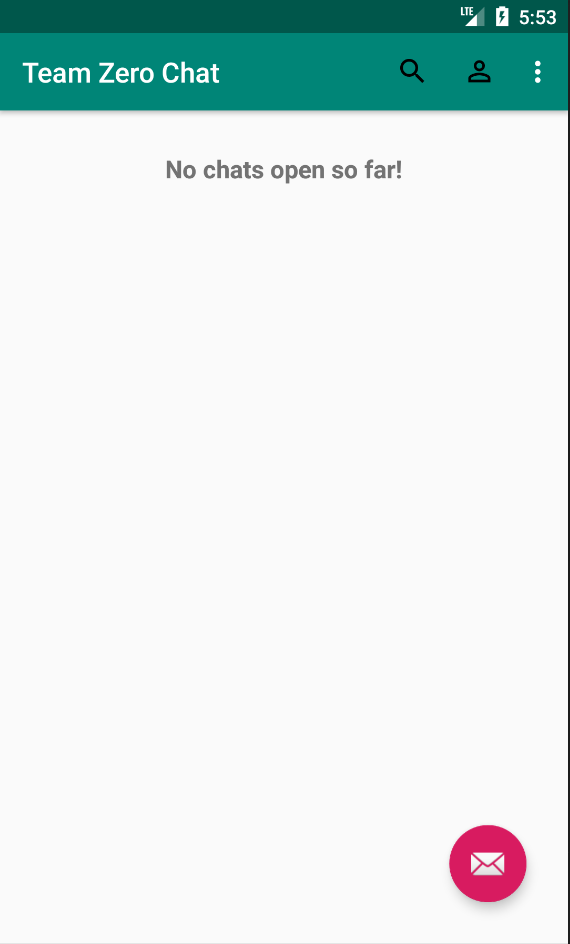
\includegraphics[width=.6\linewidth]{images/ChatList.png}
  \caption{ChatList Activity with no chats open}
  \label{chatListNoMessages}
\end{minipage}%
\begin{minipage}{.5\textwidth}
  \centering
  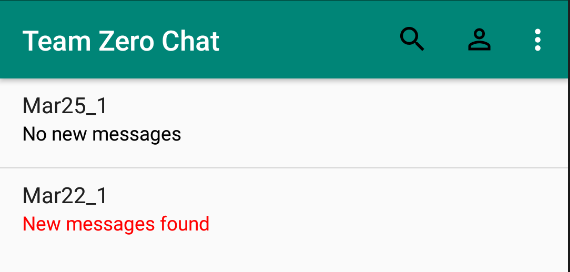
\includegraphics[width=.8\linewidth]{images/ChatListMessages.png}
  \caption{ChatList Activity with two chats open}
  \label{chatListWithMessages}
\end{minipage}
\end{figure}

% More specifically, the \verb|ListView| that contains the chats is made up of an \verb|ArrayAdapter| that has two separate lines (one for the username and one for the message status).

In order for a chat to NOT be considered as having unread messages, the user must click on the chat to view the content. This activity contains a \verb|runnable| action that checks \textbf{each 1 second} for new messages received through the WebSocket connection. Whenever there is a new message, it is put inside a variable that serves as a message queue containing the sender and messages. From that message queue, the sender is extracted and the algorithm analyses if the user currently logged in has already a chat open with the sender. If yes, it changes the status of the chat from "No new messages" to "New messages found" in red. If no, before changing the status, the new chat must be \textbf{appended to the chat list}. As part of this process, the client sends a \verb|getPublicKey| JSON request with the sender's username to find his/hers public key. Then the shared secret is calculated by using the \verb|generateSharedKey| method under the \verb|DHUtilities| class. It is then stored in the local database along with the sender's username, public key and a column named \verb|ChatBelongsTo| that must contain the receiver's username (i.e. you). The latter is \textbf{necessary} in order for the application to know which chats belong to which user logged onto the device. Without it, somebody can view view other users' chats and \textbf{access information that is not intended for him/her}.

From this activity, one can do any of the following actions:

1) Initiate a chat with a new user by clicking the red circle in the lower-right area of the screen

2) Select and open one of the user's chats that are already initiated (similar to what can be seen in figure \ref{chatListWithMessages})

3) Open up the settings in the upper-right side and select either to sign out, unregister the account, delete all the chats that are currently open or hide the chat history for this session only

Next up, we will explain the points above in the mentioned order.

\textbf{NewChat activity} (linked to the \verb|new_chat_layout.xml| front-end layout)

From this activity, the user can search for any other user that he wants to open a chat with. Upon entering this view, a sensible message appears on the screen announcing you of the steps needed to take in order to either \textbf{display all the users} (figure \ref{newChatDisplayAllUsers}) or just \textbf{search users by name} (figure \ref{newChatDisplaySelectUsers}). The resulted information is a list of users fetched from the server's database along with their \textbf{statuses} at the moment (offline/online). 

\begin{figure}[H]
\centering
\begin{minipage}{.5\textwidth}
  \centering
  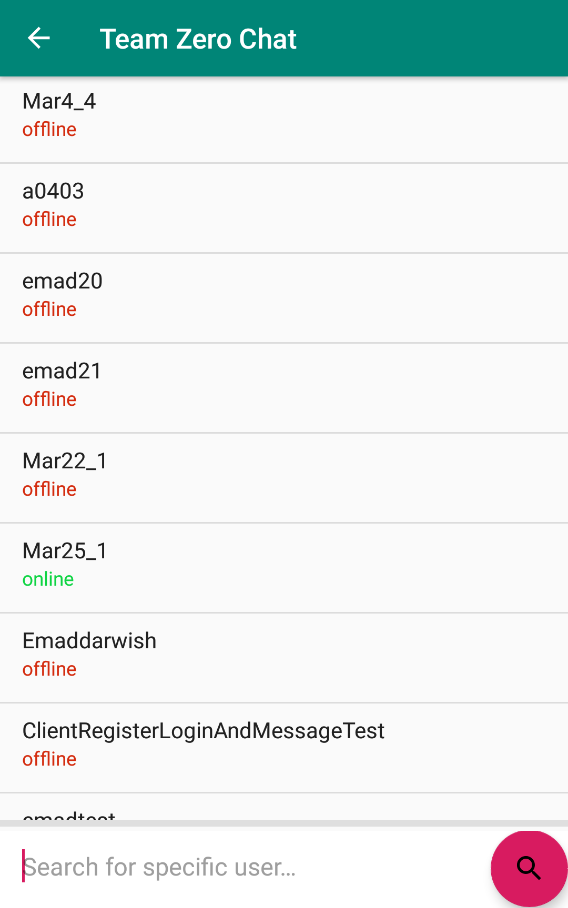
\includegraphics[width=.6\linewidth]{images/NewChatAllUsers.png}
  \caption{Display all users from the server}
  \label{newChatDisplayAllUsers}
\end{minipage}%
\begin{minipage}{.5\textwidth}
  \centering
  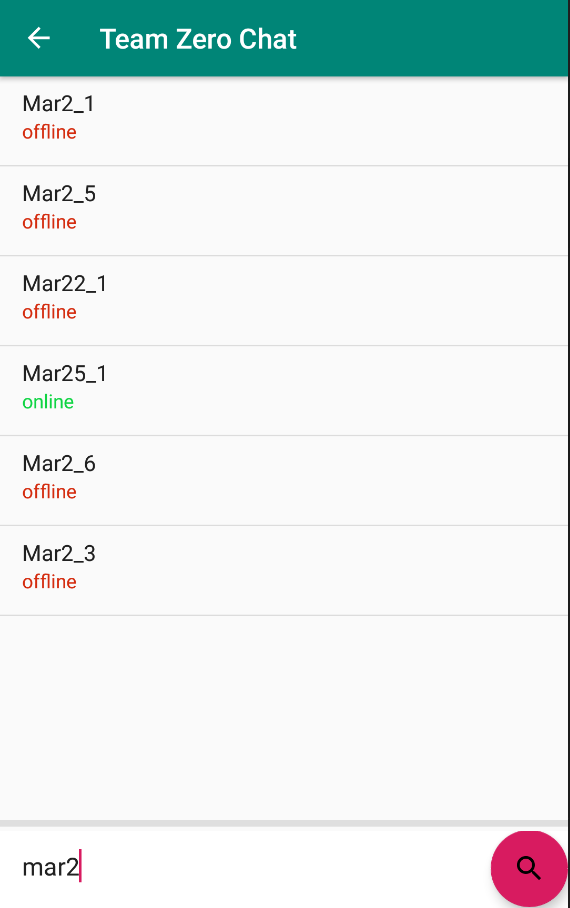
\includegraphics[width=.6\linewidth]{images/NewChatSelectUsers.png}
  \caption{Search for users}
  \label{newChatDisplaySelectUsers}
\end{minipage}
\end{figure}

If there are no registered users in the server's database or the server cannot find the username that you are searching for, our application tells you about the issue with a sensible message ("{\it{No contacts found on our database. Please try again.}}" or {\it{"No contact found with the requested name. Please try another name.}}").

From here on, the user can click on a person to initiate a chat with. The process that starts upon selection is similar to the process that takes place when receiving a message from a user that you do not have a chat with. The only difference is that because the \verb|GETALLCONTACTS| and \verb|SEARCHCONTACTS| JSON requests \textbf{already return the public keys} of the retrieved users, they are \textbf{directly stored into the local database} (no need to call \verb|GETPUBLICKEY| to fetch the public keys). After this, the view is returned to the chat list activity and the newly initiated chat can be seen in the list.

\textbf{Chat activity} (Linked to \verb|chat_layout.xml|)

The chat activity is the main point of communication between persons in the application. In here, the user can send/receive messages and view them. The figure \ref{chatExampleTwoUsers} shows an example chat between two users.

\begin{figure}[H]
 \centering
  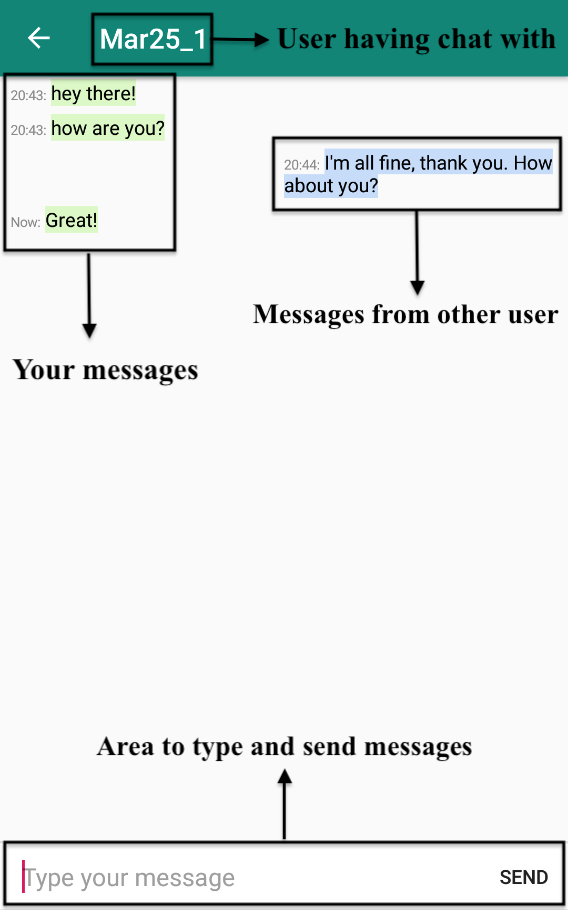
\includegraphics[width=0.3\textwidth]{images/Chat.png}
  \caption{Example chat between two users}
  \label{chatExampleTwoUsers}
\end{figure}

By default upon entering a chat, the application will execute a \verb|GETCHATHISTORY| JSON request to the server to retrieve the chat history for the \textbf{past 24 hours}. As seen on the left side of each message, there is a timestamp. \textbf{All the messages} that are currently sent or received in this session include a "Now:" in front of them. If the back button is clicked to return to the list of chats and then re-enter the same chat, the time in the format of \textbf{{\it{HH:MM}}} will appear instead (like in figure \ref{chatExampleTwoUsers}).

We have to mention that the messages received in this chat session are retrieved from a local message queue (\verb|messages| from the file \verb|UserDetails|). This queue is filled with messages received in real time by the WebSocket. If the sender of the message is this person that we are having a chat with, then just display his/her messages on screen and delete the content from the queue. This approach is much more efficient than periodically executing a \verb|GETCHATHISTORY| request from the server.

Thus, \verb|GETCHATHISTORY| is called \textbf{only once} to retrieve the history - When opening the chat session.

The messages are encrypted and decrypted using the shared secret computed from the other user's public key and your private key (step that happened either when you initiated a new chat \textbf{OR} when the other person initiated a new chat with you).

\textbf{Settings}

By clicking on the three dots sign (...) on the upper-right side of the screen with the chat lists, the user can access the settings. In there, he can do any of the following:

1) \textbf{Sign Out} - By signing out, the user is taken to the main login page upon which the app is launched on. The websocket connection is closed in order to signal the server that the user ended his online session.

2) \textbf{Unregister} - The app sends an \verb|UNREGISTER| JSON request to the server, then \textbf{deletes the user from the app's local database along with the chats owned by him}. After that, it closes the websocket connection and takes the user to the main login page.

\textbf{Important note:} before signing out or unregistering, we implemented in our code to \textbf{close the handler that checks every one second for the new messages}. We noticed that if this wouldn't have been implemented, then multiple instances of this handler were to be created when another user logs in. As they stack up, the application could've worked slower and slower until it became unresponsive and crashed.

3) \textbf{Delete All Chats} - By selecting this option, the user agrees to delete all his active chats so they no longer appear in his chat list. Deleting the chats removes all the previously stored information about them on this device, including the shared keys. However, it does \textbf{not} delete the messages that are stored on the server side.

4) \textbf{Hide Chat History} - This option allows the user to turn off (and back on) the retrieval of chat history for this current session of his online activity. By having this option on, the \verb|GETCHATHISTORY| JSON request to the server is \textbf{bypassed and not called} when entering a chat with somebody else.

\subsection{Other important implementation notes}

There is an interesting mention about the way we implemented the change of activities (i.e. going from one screen to another). We have used the \verb|setOnClickListener| method over the buttons instead of using \verb|android:onClick| at the XML level. For the latter, Android uses java reflection behind the scenes. Performance-wise, looking up a class via reflection is more computationally expensive than calling a method of the \verb|Button| class. We have used this approach throughout the whole application to avoid slowing down the performance.

We have disabled or changed the functionality of the native back button found on the lower left side of any Android device. This is important in order to \textbf{not allow the user to see sensitive information from other users that we're previously logged into the device}. This happens because the default Android button shows you \textbf{what the previous screen was}, and doesn't act like a “normal back button". For instance, if a user logged out and you click the default button, you can actually see the other user’s ChatList screen, exposing all of his chats to you. This was mitigated by bypassing this functionality with a custom one. On some activities like the launch login page or the chat list page, the default back button's functionality is disabled altogether and replaced with a sensible pop-up message. On the other activities, the button calls the \verb|onSupportNavigateUp| method. This method finishes the current activity (dismisses dialogs, closes searches etc.) and goes to the parent activity.

From a code perspective, an interesting note is that the \verb|GETCHATHISTORY|, \verb|GETALLCONTACTS| and \verb|SEARCHCONTACTS| JSON requests to the server can, sometimes, return only a single element. When returning more than one element, the JSON will contain an array delimited by square brackets ('[]'). In Java, for the array we can use a \verb|JSONArray| to fetch the data, but doing so onto a single object will result in a crash. For the latter, we have to use \verb|JSONObject| and have to cover the whole block of check into a try-catch (see lines 250-285 in \verb|Chat.java| file for example).

\subsection{WebSocket}

For the establishment of the persistent connection of the client to the server, we are using WebSocket version 1.3.0 (external library \verb|java-websocket-1.3.0|). This choice of version has been imposed across all of our platforms in order to ensure full compatibility between the clients and the server. We have also chosen this specific version because it is considered a stable and tested release, in order to increase the reliability of our system by decreasing the number of possible failures.

The websocket \textbf{is not serializable or parcelable}. In order to keep the same objects when changing activities, they need to be any of the above two. In this case, we cannot "pass" the connection from one activity to another. Because of this, we created a \textbf{handler class} (\verb|WebSocketHandler|)\textbf{with a static reference to the websocket} which we use to handle the connection and data exchange. With this approach, we can keep the connection alive during every activity in our application.

The \verb|onMessage| method adds the received messages received (either while online or offline upon login) to the message queue.

There are 2 different methods used to send messages to the server:

1) \verb|sendMessageAndWait| - Sends the message to the server and \textbf{awaits a response within a timeout period}. This method is used on requests to the server that require a response in order to proceed. A few examples include the login, registration, contact search etc. The timeout is set to 10 seconds, as we consider it a decent amount of time for a response. If the app does not receive a response within 10 seconds, it will display an appropriate message to the user telling him/her to try again.

2) \verb|sendMessage| - Sends the message to the server \textbf{without waiting for a response from it}. This method is used when sending text messages to other users, as the Android client does not need a response from the server and can continue it's actions.

\subsection{Local Database}

SQLite is at the core of our local database for the Android client. We can execute the CRUD actions directly using SQLite queries, but boilerplate code is mostly unavoidable this way. Because of this and the fact that Android Room efficiently converts tables into Java objects made the latter our primary choice.

There are multiple reasons for having a local database. One is that it stores information that does need to be passed to the server, like the private keys. Another is because of it's convenience in fetching data fast from the same device, as opposed to sending costly JSON requests to the server for each tiny information to be retrieved again (like the public keys of other users).

The figure \ref{androidLocalDatabase} displays the local database's schema.

\begin{figure}[H]
 \centering
  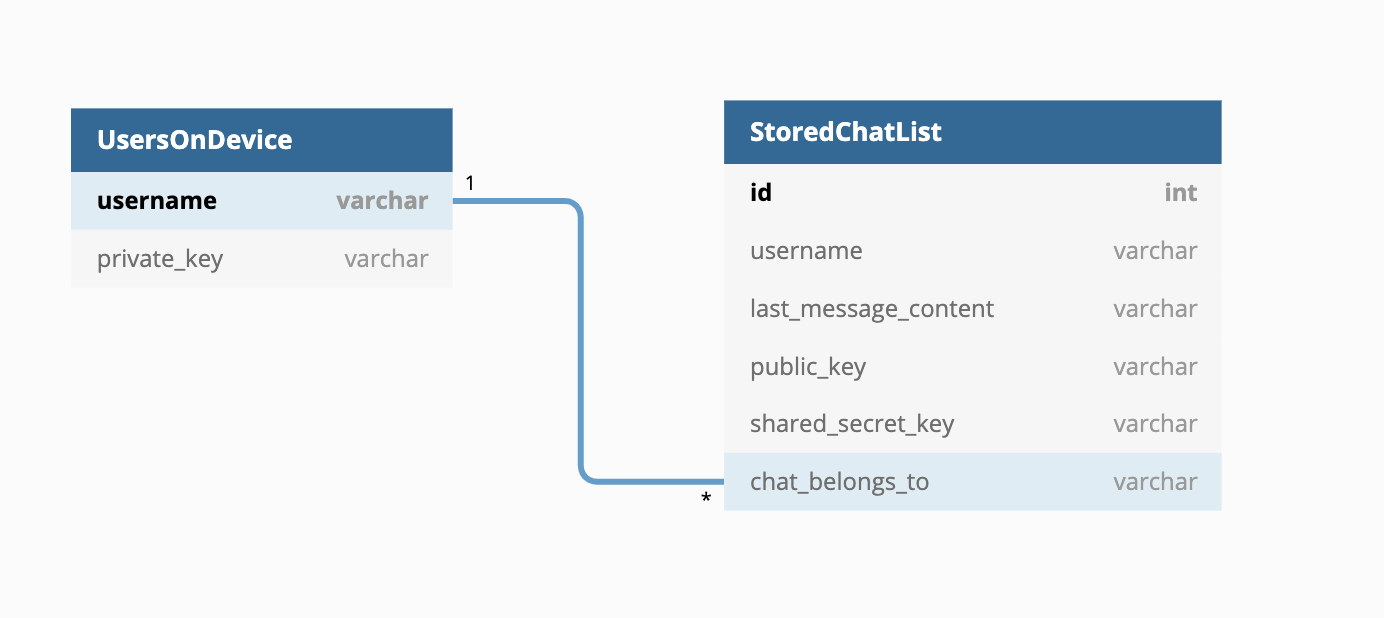
\includegraphics[width=0.8\textwidth]{images/AndroidLocalDatabase.png}
  \caption{Local Database Schema}
  \label{androidLocalDatabase}
\end{figure}

\textbf{UsersOnDevice} is the table that refers to the users registered on this device. It has the username for each user and his/her account's private key.

\textbf{StoredChatList} is the table which stores the chats for the users found in \textbf{UsersOnDevice}. \verb|id| is the primary key and it is auto-incremented after each insert. In here, the \verb|username| column refers to \textbf{the username with which} \verb|chat_belongs_to| \textbf{has a chat with}.

There is a one-to-many relation between the first table and the second one \\ (\verb|UsersOnDevice.username| $\rightarrow$ \verb|StoredChatList.chat_belongs_to|). This means that one username can have \textbf{zero, one or multiple chats} associated with his/her account.

Upon deletion of a user from this device, \textbf{all of his stored chats are deleted too}. From a technical perspective, this is accomplished by adding a {\it{cascade delete}} rule. The rule must run from \verb|UsersOnDevice| $\rightarrow$ \verb|StoredChatList| and not vice-versa. Thus, when removing username X from this device, it will automatically remove all the chats in \verb|StoredChatList| where \verb|chat_belongs_to| = X.

All of the operations that run on the local database are \textbf{completed as a background tasks}. The reason why is because each operation blocks the current thread on which it executes until it finishes. By running all the database operations on the main thread, the application will be greatly slowed down and the UI may remain locked for that period.

\subsection{Internal Tools}

\textbf{RegistrationValidator} is, as already explained in the chapter \ref{android-implementation}, the tool with which the login and registration fields are validated (figures \ref{tab:login_validations} and \ref{tab:registration_validations}). RFC5322 is the latest internet message format protocol that provides the formal definition of e-mail addresses \cite{RFC8322-e-mail}. We must mention the fact that our e-mail validation is \textbf{not fully RFC5322 compliant}. For instance, it does not accept e-mail addresses that contain single quotation marks (') like {\it{test'name@test.com}}. It also does not accept e-mail addresses that do not end with .[name], like {\it{admin@mailserver}}. However, it accepts most of the regularly used e-mail addresses and reject potentially malicious code like SQL injection. A full list of our tests will be displayed in the next chapter (\ref{android_unit_instrumented_testing}).

\textbf{JSONConstructor} is an internal tool that we've created to \textbf{easily construct JSONs} for requests sent to the server. It is a class which contains methods for each JSON request used in the distributed chat system. Let's consider the following example for the \verb|REGISTER| request (figure \ref{jsonConstructExample}).

\begin{figure}[H]
 \centering
  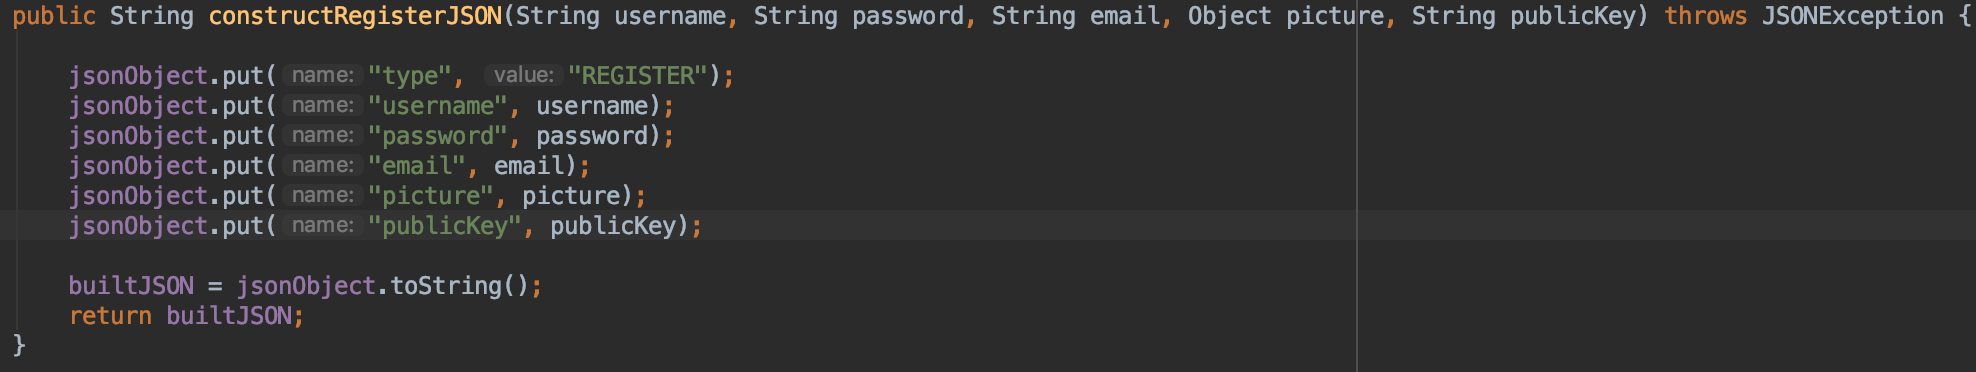
\includegraphics[width=0.9\textwidth]{images/JSONConstruct.png}
  \caption{Register JSON request construction}
  \label{jsonConstructExample}
\end{figure}

The method's arguments represent the values for each key. They are then used as 2nd arguments for the \verb|put| method of \verb|JSONObject| to form the JSON that will be sent to the server. We consider this an easier and more effective way to write code because the methods can be called in our activities whenever needed in a single line of code each.

\textbf{UserDetails / OtherUsersData} are files that store temporary information than can be used immediately. The first file contains fields related to the user currently logged in (like his username, who is he chatting with right now, his messages or is the history is hidden for this session). The latter serves as an intermediate way of passing information to the local database in an OOP fashion. For example, the information received from the server when the user initiates a new chat with another user, like the public key, is then stored temporary in an object of \verb|OtherUsersData|. It is then retrieved from there only when (and if) needed. This is a good thing to have because you may try to get a contact to chat with but then you change your mind, so the information must not get (yet) into the local database unless confirmed (by clicking the user you want to chat with from the list).

\textbf{Encryption utility files} include the following:

1) RFC5114KeyData - Contains the prime numbers P and Q in hexadecimal form that are used for the key generation with Diffie-Hellman.

2) DHUtilities - Contains the methods to generate public and private keys using prime numbers from \verb|RFC5114KeyData| file. It also contains the method that computes the shared secret between one public and one private key and 2 methods that transform a Base64 string into a public key. The latter is needed because the transmission to/from the server of public keys is done in Base64, so they need to be converted to the appropriate data type after.

3) AES256Cryptor - Is the filed that contains the encryption and decryption algorithm for our end to end protocol. It is done in AES CBC on 256 bits. More details about encryption in chapter \ref{encryption}.

\subsection{Unit Testing \& Instrumented Testing}
\label{android_unit_instrumented_testing}

We have executed several tests upon the mobile application to ensure the functionality and usability of the client. Other than the manual tests that have been executed every time after a feature was implemented, we have conducted a series of unit and instrumented tests on a few of the features.

The file \verb|RegistrationUnitTests.java| contains a series of \textbf{unit tests} specifically targeted at validations. They check for expected correct values, like a proper password with a decent strength (at least 1 uppercase, at least one special character etc.) and also for incorrect values that can have potentially harmful behaviour.

The following list includes a few examples of potentially harmful commands: \\
"\verb|"'OR 1=1--"@gmail.com|", "\verb|'OR 1=1--@gmail.com|", "\verb|'or 1=1-@gmail.com|", \\
"\verb|1'or'1'='1|", "\verb|' or 'a'='a|", "\verb|" or "a"="a|", "\verb|') or ('a'='a|", "\verb|") or ("a"="a|". They all can trigger an SQL injection attack to the server and it is the best to filter it out directly from the input, not only at server level.

In regards to the e-mail addresses, we have successfully tested the following types of formats in JUnit and they all work on our system: "\verb|lowercase@lc.com|", "\verb|UPPERCASE@UC.COM|", "\verb|eMaIL@EmAiL.cOm|", "\verb|test@email.co.uk|", "\verb|lowercase\_@UPPERCASE.COM|", \\ "\verb|email+100@email.com|", "\verb|email+100@e-mail.co.uk|".

% Made the Toasts that appear on registration page outside the methods (i.e. in Registration activity). Otherwise, unit tests wouldn't have been possible because getApplicationContext() used for Toast creation is not mocked

\textbf{JSONConstructionInstrumentedTests} includes the automated tests for the JSON request construction. It is used to generate multiple types of JSONs in various situations and compare its output to what is expected on the server end.

\subsection{Current Drawbacks}

Upon registration of a new user, a new set of public and private keys are generated using \verb|java.security.KeyPair|. The keys work for encryption and decryption between the same client (Android), but do not work when trying to chat with the web client. This happens because the generated keys in Base64 in \verb|java.security| (Android client) are of different size than the keys generated in Base64 in \verb|CryptoJS| (web client). Because there are discrepancies between the clients in the way the keys are generated, we have decided as a trade-off to use a sample set of keys generated using the web client's CryptoJS library. More information about the encryption in the chapter \ref{encryption}.

Right now, the same user can be added more than once in the chat list. This does not disrupt the application in the way it functions, but you can see multiple chats with user A if you choose to initiate more than one chat with A (and they all contain the same chat history). This can be mitigated by querying the local database in order to check if that user already exists or not in your chat list.

Every time a user enters a chat, it retrieves the chat history by sending a JSON request to the server. It is not the most efficient approach because it's an expensive operation in regards to time passed. It is better to store the messages in the local database.

As backwards compatibility comes to mind, clients that did not register on this specific Android device cannot chat. This happens because after logging in and either receiving messages or initiating a new chat, the app tries to retrieve the private key of the user. Because the server does not get/send private keys and the mobile devices does not have the private key, it will result in a crash.

% There is a small chance that at login, when the user receives messages that were sent to him while being offline, those messages would appear in the websocket queue before the LOGIN response from the server appears. This would not make the application crash and nor the login process fail, but it will make it much slower. Particularly, it will freeze for 10 seconds. This is the time it takes for the TimeoutException of the concurrent thread to be thrown. --> This was managed to be partially solved by adding a small delay when sending messages to the client that were received while being offline. The delay would not add up for the server and does not pose a scalability problem because it works on different threads, so basically just one thread on the server would be affected by the small delay (which is hard-coded to 10 ms).

\subsection{Further Improvements}

The status of the internet connection can be monitored by using different methods found in \verb|android.net.ConnectivityManager|. It can be a good idea to send broadcast intents when the network connectivity is lost so the user is notified of the problem (and remain on a buffering screen so that the user comprehends that the application is doing background work while reconnecting to the internet). If the user wants to close the application, it's also possible to store the ID of the last screen onto which the user was interacting, in the local database. This is possible because the local database can be accessed with or without the internet connection. After the app is opened again and the internet connection is live, it can resume from the stored checkpoint. The permissions that are being used for these actions are \verb|ACCESS_NETWORK_STATE| and \verb|ACCESS_WIFI_STATE| (the latter is useful for accessing the \verb|android.net.wifi.WifiManager| that manages all aspects of the WiFi connectivity in particular). They are already inserted in the Manifest file of the application and require using the \verb|getActiveNetworkInfo| method over the \verb|ConnectivityManager| to check the connection status.

Adding the possibility to retrieve the chat history for any amount of time the user wants to. It can take the form of a new element in the drop-down list of the settings named "Chat History Time" and then the user can select from a spinner the number of hours/days to retrieve the history from.

In regards to the chat history hide mode, if user A turns off the chat history and logs back in, it will automatically be on again. A possibly better implementation would be to register in the local database the choices made by this particular user and know it for further usage (i.e. remember his choice when he logs back in).

The "remember login credentials" check from the login page does not have the functionality implemented yet. It can be implemented by adding another column to the \verb|UsersOnDevice| table to store if the check is on or off. If it is on, then it can automatically login back into the account until the user explicitly signs out and the flag is turned to {\it{false}}.
\label{android}


\section{Encryption}
\label{encryption}
The chat messages in Team Zero Chat Application that the clients sent each other are encrypted end-to-end using various protocols. We decided to use a public-key exchange protocol to allow clients to communicate securely without having been in direct contact with one another previously. However, as public-key cryptography is both resource intensive and asymmetric (therefore only allowing decryption of one-sided messages) we decided to use a symmetric key and algorithm for the encryption and decryption of the chat messages themselves. The entire encryption process is detailed below.

\subsection{Diffie–Hellman key exchange}

\subsubsection{Public and private key generation}

Each client, before registering with the server, uses Diffie-Hellman key exchange protocol algorithms to generate a public and private key unique to the user\cite{rfc2631}. The public key is converted to a base64 string and sent to the server on registration, so that other clients can access it as well. The private key is stored locally for both of our implemented clients.

\subsubsection{Key agreement protocol}

When starting a new chat, the initiating client retrieves the public key of the receiving client from the server and converts it from base64 to the appropriate data type required by either Java (Android) or JavaScript (web client). After this step, the Diffie-Hellman Key agreement protocol's algorithm that generates the shared key\cite{rfc2631} is used with the \textbf{initiating client's private key} and \textbf{receiving client's public key} to compute a \textbf{shared secret}.

The generated keys use the same prime numbers Q and P (base and modulus numbers) on both platforms. This is required because if the prime numbers are randomly generated, then the resulted keys will not produce the same shared secret when computed.

Using the same algorithm of the Diffie-Hellman key exchange protocol, the receiving client will compute \textbf{the same shared secret key} with the initiating client's public key and their own private key, once they receive a message notification. After this, the generated shared secret is then used as input passphrase to the encryption and decryption of our end-to-end protocol (AES CBC on 256 bits).

In regards to the actual implementation on the clients, we have encountered one problem. The \verb|KeyPairGenerator| object found in \verb|java.security| (used in the Android client) does not generate keys of the same size as in \verb|Crypto| (used in the Web client). Even though the prime numbers for the generator are the same in both clients and the algorithm generates the keys using 512 bits, the results are of different length in each platform. This results in the inability to generate the same shared secret between different platforms \textbf{but} can successfully generate the same shared secret between same client types. To overcome this issue, we have decided to temporarily select (hardcode) private and public keys according to the Web client's method, instead of using the cryptographic algorithms to generate them. While this decreases the security of the system, it allows for proof-of-concept implementation of the rest of the encryption protocols, until a solution can be found.

\subsection{Advanced Encryption Standard CBC}

Our algorithm of choice for the end-to-end encryption and decryption of messages is AES (Advanced Encryption Standard). The mode of operation that we have used for AES is CBC (Cipher Block Chaining). It was invented in 1976 by William F. Ehrsam, Carl H. W. Meyer, John L. Smith, and Walter L. Tuchman \cite{aes-cbc-patent}. This mode stands behind the classic Blockchain algorithm that is widely used in cryptocurrencies. Each block of plaintext is XOR-ed with the previous cipherblock before being encrypted. By using this mode, each new ciphertext block depends on \textbf{all the plaintext blocks processed up to that point}. In order to make each message unique, the first block that is constructed must use an initialization vector (IV), which is a fixed size random or pseudo-random number. 


The computed shared secret by the Diffie-Hellman algorithm (called a "passphrase") is used as the key for the AES encryption and decryption. One important note is that we have used \textbf{256 bits} for both clients for encryption/decryption. An advantage to using AES CBC is that for the same message (plaintext), \textbf{a different encrypted text (ciphertext) is generated every time}. With this method, all chat messages between two parties can be securely sent.

\subsection{Encryption in group chats}
\label{encryption-groups}
Group chats are currently not encrypted. However, two methods with which group chat encryption could be implemented are discussed here.

\subsubsection{Method 1 - Multiple end-to-end messages}
Currently when a user sends a message to a group chat, it is sent to the server as a single message, and sent from the server to recipients as multiple messages. 

With this encryption method, the sending user would need to send \textit{n} number of separate encrypted text messages for a group message in a group of \textit{n} members. The message would need to be encrypted with the shared secret key derived with the above algorithms from each group member's public key. Thus sending a group message to a group of 10 users would be similar to sending 10 regular chat messages. This is similar to how group messages work in the Signal protocol\cite{signal_groups}, which is what WhatsApp and Facebook Messenger use.

This method, while very secure, involves having to fetch client keys and encrypt the a message multiple times.

\subsubsection{Method 2 - Group creator generates and shares key}

This is a less computationally expensive method, but where there is more responsibility on one client than others.

The client who creates the group chat would generate a 256 bit AES key that can be used as a shared secret key for encryption and decryption. This will become the group's key. Whenever a new member joins the group, the creator will securely send the secret key via asymmetric encryption methods (using the new member's public key to encrypt it, so only the new member's private key can decrypt it). Therefore, all joining members will have the shared key to encrypt and decrypt messages with, and members will only have to send a message once.

However, a notification system will need to be implemented to notify the remaining members of a group once a user leaves a group, as the group creator would need to generate and distribute a new key.

